\chapter{Komponentensemantik}

\begin{figure}[hbt]
  \centering
  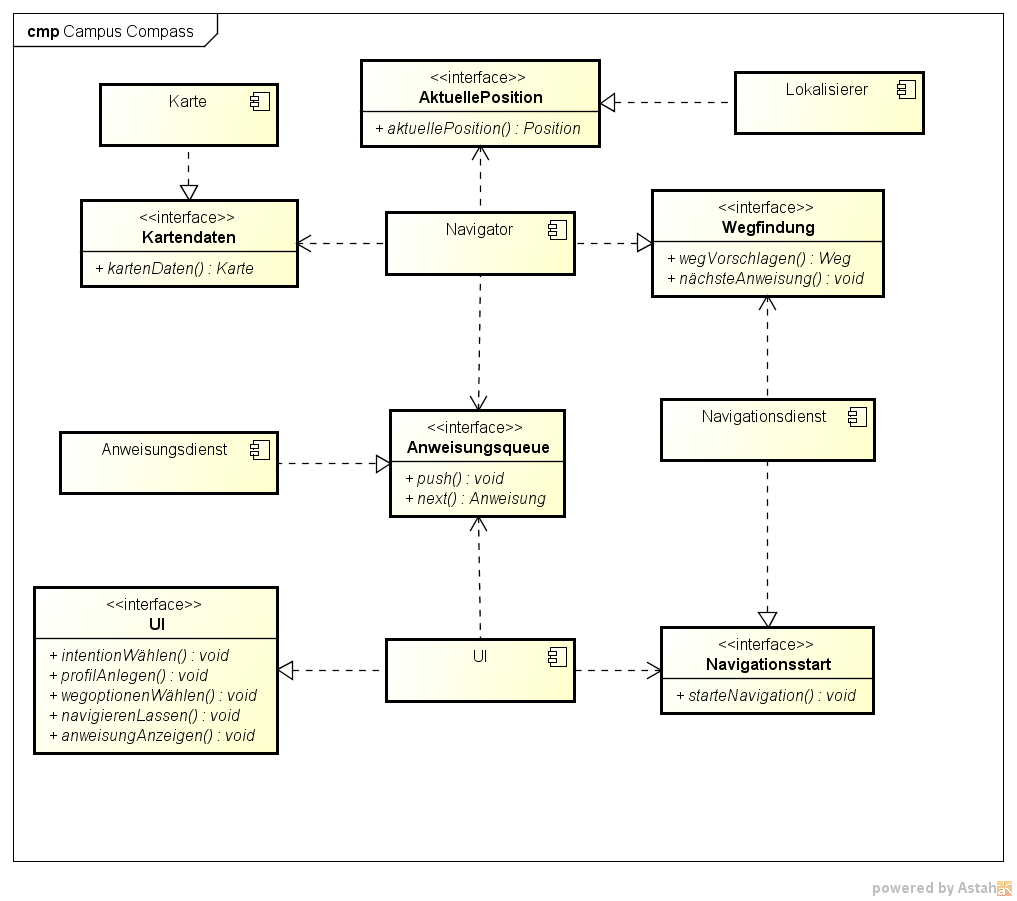
\includegraphics[width=\linewidth]{img/komponentendiagramm_neu.png}
  \caption{Komponentendiagramm explizite Schnittstellen}
\end{figure}

Das Komponentendiagramm in der externen Sicht zeigt die Komponenten und ihre
Interfaces. Hieran lässt sich besonders gut sehen, welche Komponenten des
Systems austauschbar sind und welche Interfaces die Komponenten implementieren
müssen. Der User interagiert in unserem System auschließlich mit dem
UI-Interface und ist damit klar vom restlichen System getrennt.
